\documentclass{article}
\usepackage{ae,aecompl}
\usepackage{todonotes}
\usepackage{chngcntr}
\usepackage{tikz-cd}
\usepackage{graphicx}
\graphicspath{ {./images/}}
\usepackage[all,cmtip]{xy}
\usepackage{amsmath, amscd}
\usepackage{amsthm}
\usepackage{amssymb}
\usepackage{amsfonts}
\usepackage{bm}
\usepackage{qsymbols}
\usepackage{latexsym}
\usepackage{mathrsfs}
\usepackage{mathtools}
\usepackage{cite}
\usepackage{color}
\usepackage{url}
\usepackage{enumerate}
\usepackage{verbatim}
\usepackage[draft=false, colorlinks=true]{hyperref}
\usepackage{pdfpages}
\usepackage[margin=1.2in]{geometry}
\usepackage{IEEEtrantools}

\usepackage{fancyhdr}


\usepackage[nameinlink]{cleveref}


\DeclareMathOperator*{\ac}{accept}
\DeclareMathOperator*{\amax}{argmax}
\DeclareMathOperator*{\amin}{argmin}
\DeclareMathOperator*{\Aut}{Aut}
\newcommand {\al}{{\alpha}}
\newcommand {\abs}[1]{{\left\lvert#1\right\rvert}}
\newcommand {\A}{{\mathcal{A}}}
\newcommand {\AM}{{\mathrm{AM}}}
\newcommand {\AMp}{{\AM_{p}^{X}\!(\Ri_\w)}}
\newcommand {\B}{{\mathcal{B}}}
\DeclareMathOperator*{\Be}{Bern}
\newcommand {\Br}{{\dot{B}}}
\newcommand {\Ba}{{\mathfrak{B}}}
\newcommand {\C}{{\mathbb C}}
\newcommand {\ce}{\mathrm{c}}
\newcommand {\Ce}{\mathrm{C}}
\newcommand {\Cc}{\mathrm{C_{c}}}
\newcommand {\Ccinf}{\mathrm{C_{c}^{\infty}}}
\DeclareMathOperator{\cov}{Cov}
\DeclareMathOperator{\DEV}{DEV}
\newcommand {\Di}{{\mathbb D}}
\newcommand {\dom}{\mathrm{dom}}
\newcommand{\dist}{\stackrel{\mathrm{dist}}{=}}
\newcommand {\ud}{\mathrm{d}}
\newcommand {\ue}{\mathrm{e}}
\newcommand {\eps}{\varepsilon}
\newcommand {\veps}{\varepsilon}
\newcommand {\vrho}{{\varrho}}
\newcommand {\E}{{\mathbb{E}}}
\newcommand {\Ec}{{\mathcal{E}}}
\newcommand {\Ell}{L}
\newcommand {\Ellp}{{L_{p}[0,1]}}
\newcommand {\Ellpprime}{{L_{p'}([0,1])}}
\newcommand {\Ellq}{{L_{q}([0,1])}}
\newcommand {\Ellqprime}{{L_{q'}([0,1])}}
\newcommand {\Ellr}{L^{r}}
\newcommand {\Ellone}{{L_{1}([0,1])}}
\newcommand{\Elltwo}{{L_{2}([0,1])}}
\newcommand{\Ellinfty}{L^{\infty}}
\newcommand{\Ellinftyc}{L_{\mathrm{c}}^{\infty}}
\newcommand{\exb}[1]{\exp\left\{#1\right\}}
\DeclareMathOperator*{\Ext}{Ext}
\newcommand{\F}{{\mathcal{F}}}
\newcommand{\Fe}{{\mathbb{F}}}
\newcommand{\G}{{\mathcal{G}}}
\newcommand{\HF}{\mathcal{H}_{\text{FIO}}^{1}(\Rd)}
\newcommand{\Hr}{H}
\newcommand{\HT}{\mathcal{H}}
\newcommand{\ui}{\mathrm{i}}
\newcommand{\I}{{I}}
\newcommand{\J}{{\mathcal{J}}}
\newcommand{\id}{{\mathrm{id}}}
\newcommand{\iid}{\stackrel{\mathclap{\normalfont\mbox{iid}}}{\sim}}
\newcommand{\im}{{\text{im }}}
\newcommand{\ind}{{\perp\!\!\!\perp}}
\DeclareMathOperator*{\Int}{int}
\newcommand{\intx}{{\overline{\int_{X}}}}
\newcommand{\inte}{{\overline{\int_{\E}}}}
\newcommand{\la}{\lambda}
\newcommand{\rb}{\rangle}
\newcommand{\lb}{{\langle}}
\newcommand{\La}{\Lambda}
\newcommand{\calL}{{\mathcal{L}}}
\newcommand{\lp}{{\mathcal{L}}^{p}}
\newcommand{\lpo}{{\overline{\mathcal{L}}^{p}\!}}
\newcommand{\Lpo}{{\overline{\Ell}^{p}\!}}
\newcommand{\M}{{\mathbf{M}}}
\newcommand{\Ma}{{\mathcal{M}}}
\newcommand{\N}{{{\mathbb N}}}
\newcommand{\Na}{{{\mathcal{N}}}}
\newcommand{\norm}[1]{\left\|#1\right\|}
\newcommand{\normm}[1]{{\left\vert\kern-0.25ex\left\vert\kern-0.25ex\left\vert #1 
    \right\vert\kern-0.25ex\right\vert\kern-0.25ex\right\vert}}
\newcommand{\Om}{{{\Omega}}}
\newcommand{\one}{{{\bf 1}}}
\newcommand{\pic}{\text{Pic }}
\newcommand{\ph}{{\varphi}}
\newcommand{\Pa}{{\mathbb{P}}}
\newcommand{\Po}{{\mathcal{P}}}
\newcommand{\Q}{{\mathbb{Q}}}
\newcommand{\R}{{\mathbb R}}
\newcommand{\Rd}{{\mathbb{R}^{d}}}
\DeclareMathOperator{\rej}{reject }
\newcommand{\Rn}{{\mathbb{R}^{n}}}
\newcommand{\cR}{{\mathcal{R}}}
\newcommand{\Rad}{{\mathrm{Rad}}}
\newcommand{\ran}{{\mathrm{ran}}}
\newcommand{\Ri}{{\mathrm{R}}}
\newcommand{\supp}{{\mathrm{supp}}}
\newcommand{\Se}{\mathrm{S}}
\newcommand{\Sp}{S^{*}(\Rn)}
\newcommand{\St}{{\mathrm{St}}}
\newcommand{\Sw}{\mathcal{S}}
\newcommand{\T}{{\mathcal{T}}}
\newcommand{\ta}{{\theta}}
\newcommand{\Ta}{{\Theta}}
\newcommand{\topp}{\stackrel{p}{\to}}
\newcommand{\todd}{\stackrel{d}{\to}}
\newcommand{\toL}[1]{\stackrel{L^{#1}}{\to}} 
\newcommand{\toas}{\stackrel{a.s.}{\to}}
\DeclareMathOperator{\V}{Var}
\newcommand {\w}{{\omega}}
\newcommand {\W}{{\mathrm{W}}}
\newcommand {\Wnp}{\text{$\mathrm{W}$\textsuperscript{$n,\!p$}}}
\newcommand {\Wnpeq}{\text{$\mathrm{W}$\textsuperscript{$n\!,\!p$}}}
\newcommand {\Wonep}{\text{$\mathrm{W}$\textsuperscript{$1,\!p$}}}
\newcommand {\Wonepeq}{\text{$\mathrm{W}$\textsuperscript{$1\!,\!p$}}}
\newcommand {\X}{{\mathcal{X}}}
\newcommand {\Z}{{{\mathbb Z}}}
\newcommand {\Za}{{\mathcal{Z}}}
\newcommand {\Zd}{{\Z[\sqrt{d}]}}
\newcommand {\vanish}[1]{\relax}

\newcommand {\wh}{\widehat}
\newcommand {\wt}{\widetilde}
\newcommand {\red}{\color{red}}

% Distributions
\newcommand{\normal}{\mathsf{N}}
\newcommand{\poi}{\mathsf{Poisson}}
\newcommand{\bern}{\mathsf{Bernoulli}}
\newcommand{\bin}{\mathsf{Binomal}}
\newcommand{\multi}{\mathsf{Multinomial}}
\newcommand{\Exp}{\mathsf{Exp}}



% put your command and environment definitions here




% some theorem environments
% remove "[theorem]" if you do not want them to use the same number sequence


  \newtheorem{thrm}{Theorem}
  \newtheorem{lemma}{Lemma}
  \newtheorem{prop}{Proposition}
  \newtheorem{cor}{Corollary}

  \newtheorem{conj}{Conjecture}
  \renewcommand{\theconj}{\Alph{conj}}  % numbered A, B, C etc

  \theoremstyle{definition}
  \newtheorem{defn}{Definition}
  \newtheorem{ex}{Example}
  \newtheorem{exs}{Examples}
  \newtheorem{question}{Question}
  \newtheorem{remark}{Remark}
  \newtheorem{notn}{Notation}
  \newtheorem{exer}{Exercise}




\title{STATS300A - Lecture 15}
\author{Dominik Rothenhaeusler\\ Scribed by Michael Howes}
\date{11/10/21}

\pagestyle{fancy}
\fancyhf{}
\rhead{STATS300A - Lecture 15}
\lhead{11/10/21}
\rfoot{Page \thepage}

\begin{document}
\maketitle
\tableofcontents
\section{Motivation}
Today we are going to start to develop optimal two-sided tests in one-dimensional exponential families. A UMP test need not exist in this case. Indeed, in the Gaussian model with known variance and unknown mean $\ta$ there is no UMP test for $H_0 : \ta =\ta_0$ against $H_1 : \ta \neq \ta_0$. This is because for an alternative $\ta_1 > \ta_0$, the MP test rejects $H_0$ when our data is large. However for the alternative $\ta_1' < \ta_0$ the MP test rejects $H_0$ when our data is small (see picture below).

\begin{center}
    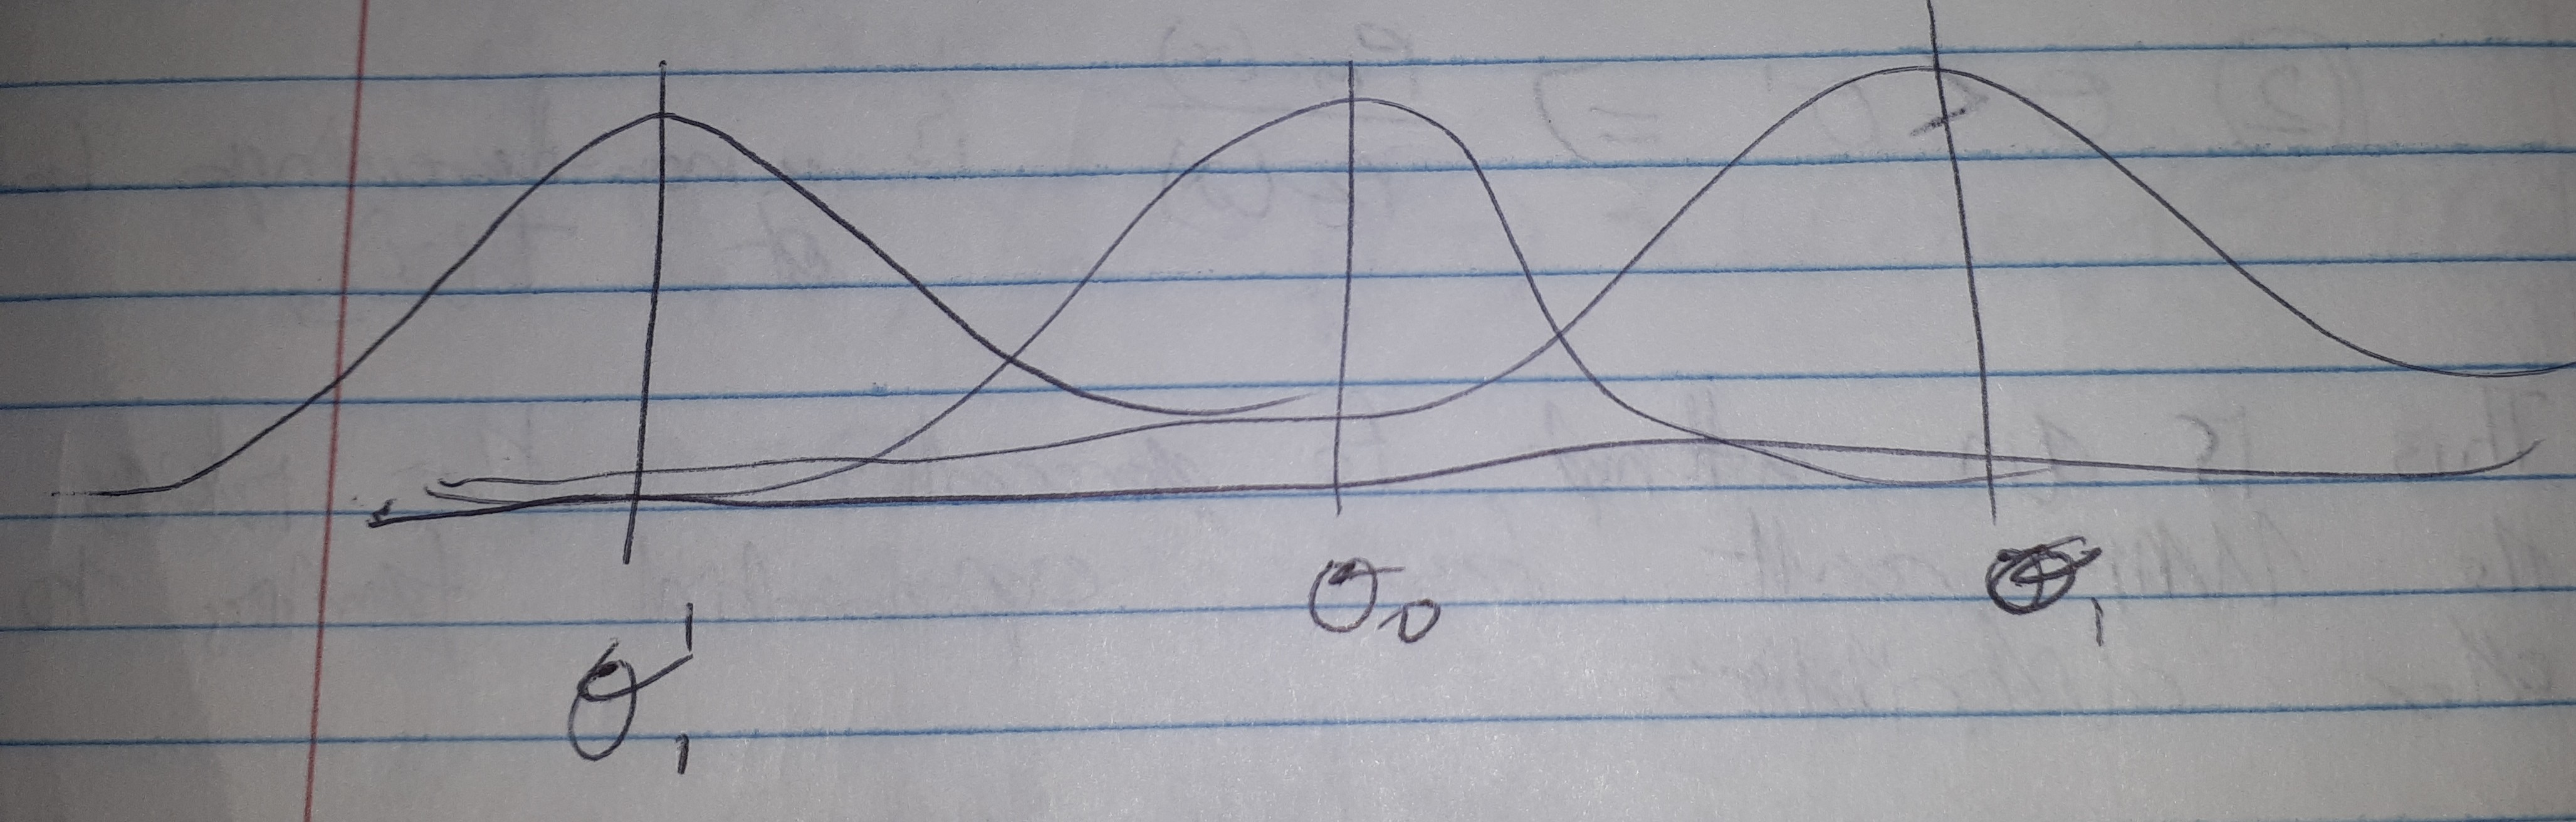
\includegraphics[width = 0.7\textwidth]{11_10_P1.jpg}
\end{center}


There are various approaches that can be used when the UMP test does not exist. These include:
\begin{enumerate}
    \item Symmetry constraints on tests. For example $\phi (c x) = \phi(x)$ for $c >0$.
    \item Put a probability distribution on $\Om_1$. Then collapse the risk function and maximize the average power.
    \item Maximize the worst case power (maximin test).
    \item Monotonicity constraints.
    \item Unbiasedness.
\end{enumerate}

We will use the last approch (unbiasedness) but it is good to know that there are other method available. 
\section{Unbiased tests}
\begin{defn}
    A test $\phi$ is \emph{unbiased} at level $\al$ if
    \begin{enumerate}
        \item For all $\ta_0 \in \Om_0$, $\E_{\ta_0} \phi \le \al$.
        \item For all $\ta_1 \in \Om_1$, $\E_{\ta_1} \phi \ge \al$.
    \end{enumerate}
\end{defn}
\begin{remark}
    Some remarks on the above definition
    \begin{itemize}
        \item This is a form of risk unbiasedness. It corresponds to having level $\al$ and being risk unbiased under 0-1 loss.
        \item UMP tests (if they exist) are always unbiased tests.
        \item Recommending reading: ``\href{https://arxiv.org/abs/1410.2597}{Optimal inference after model selection}'' by Fiftian, Sun and Taylor. This is a recent paper that uses ideas of unbiased tests.
    \end{itemize}
\end{remark}
The definition of unbiased gives us a new optimality condition. 
\begin{defn}
    A \emph{uniformly most power unbiased (UMPU) test} is an unbiased level $\al$ test which is uniformly most powerful among all unbiased level $\al$ tests.
\end{defn}
Thus we are restricting our set of tests. We have 
\[\text{unbiased level $\al$ tests} \subsetneq \text{all level $\al$ tests}. \]
A UMPU test is a test in the first class which is uniformly optimal in the first class. Unlike UMP tests, UMPU tests often exist for testing $H_0 : \ta =\ta_0$ against $H_1 : \ta \neq \ta_0$ and for testing $H_0 : \ta \le \ta_0$ against $H_1 : \ta > \ta_0$ in the presence of nuisance parameters.
\section{Constructing UMPU tests}
\subsection{A recipe}
Constructing UMPU tests is not a straight forward procedure. The general recipe that we will use is
\begin{enumerate}
    \item Rewrite constraints as weaker constraints. That is, replace unbiasedness with something weaker.
    \item Fix a simple alternative $\ta_1 \in \Om_1$.
    \item Find a MP under the constraints from (a). This will require a generalized Neyman Pearson lemma. Call this test $\phi_{\ta_1}$.
    \item If the test $\phi = \phi_{\ta_1}$ does not depend on $\ta_1$, then $\phi$ is in fact the UMP under the constraints in (a).
    \item Show that $\phi$ actuallly satisfies the stronger constraint (i.e. show $\phi$ is unbiased) and thus conclude that $\phi$ is UMPU.
\end{enumerate}
We will now work on each of the ingredients.
\subsection{$\al$-similar tests}
Typically $\Om_0$ and $\Om_1$ are subsets of $\R^k$ and so we can define 
\[W = \overline{\Om}_0 \cap \overline{\Om}_1, \]
where $\overline{A}$ is used to denote the closure of $A \subseteq \R^k$. 
\begin{exs}
    Two examples to keep in mind are
\begin{itemize}
    \item If we have the test $H_0: \ta = \ta_0$ against $H_1 : \ta \neq \ta_0$, then $W = \{\ta_0\}$.
    \item If we have the test $H_0 : \ta_1 \le \wt{\ta}$ against $H_1 : \ta_1 > \wt{\ta}$ where $\ta = (\ta_1,\ldots, \ta_k) \in \R^k$, then \[W = \{\ta \in \R^k : \ta_1 = \wt{\ta}\}.\]
\end{itemize}
\end{exs}
\begin{defn}
    A test $\phi$ is \emph{$\al$-similar} if $\E_\ta \phi = \al$ for all $\ta \in W$.
\end{defn}
\begin{lemma}
    Suppose that the function $\beta_\phi(\ta) = \E_\ta \phi$ is continuous on $\Om$ for all test functions $\phi$. If a test $\phi_0$ is UMP among all $\al$-similar tests, then $\phi_0$ is also UMP among all unbiased test.
\end{lemma}
\begin{proof}
    We will first show that $\phi_0$ is unbiased. Consider the constant test $\phi = \al$. The test $\phi$ is $\al$-similar. Since $\phi_0$ is UMP among all $\al$-similar tests we must have that for all $\ta_1 \in \Om_1$,
    \[\E_{\ta_1}\phi_0 \ge \E_{\ta_1} \phi = \al. \]
    Thus $\phi_0$ is unbiased at level $\al$. To show that $\phi_0$ is the UMPU test, it suffices to show that every unbiased test is a level $\al$ test. Since $\phi_0$ is unbiased and optimal among $\al$-similar tests, $\phi$ will thus be optimal among unbiased tests. If $\phi$ is unbiased, then by continuity of $\beta_\phi$ we have that 
    \[\E_{\ta} \phi = \beta_\phi(\ta) \le \al,~~~\text{for all } \ta \in \overline{\Om}_0. \]
    Likewise,
    \[\E_{\ta} \phi = \beta_\phi(\ta) \ge \al,~~~\text{for all } \ta \in \overline{\Om}_1. \]
    Thus $\E_\ta \phi = \al$ for all $\ta \in W = \overline{\Om}_0 \cap \overline{\Om}_1$.
\end{proof}
The idea behind this proof is that we have shown:
\begin{center}
    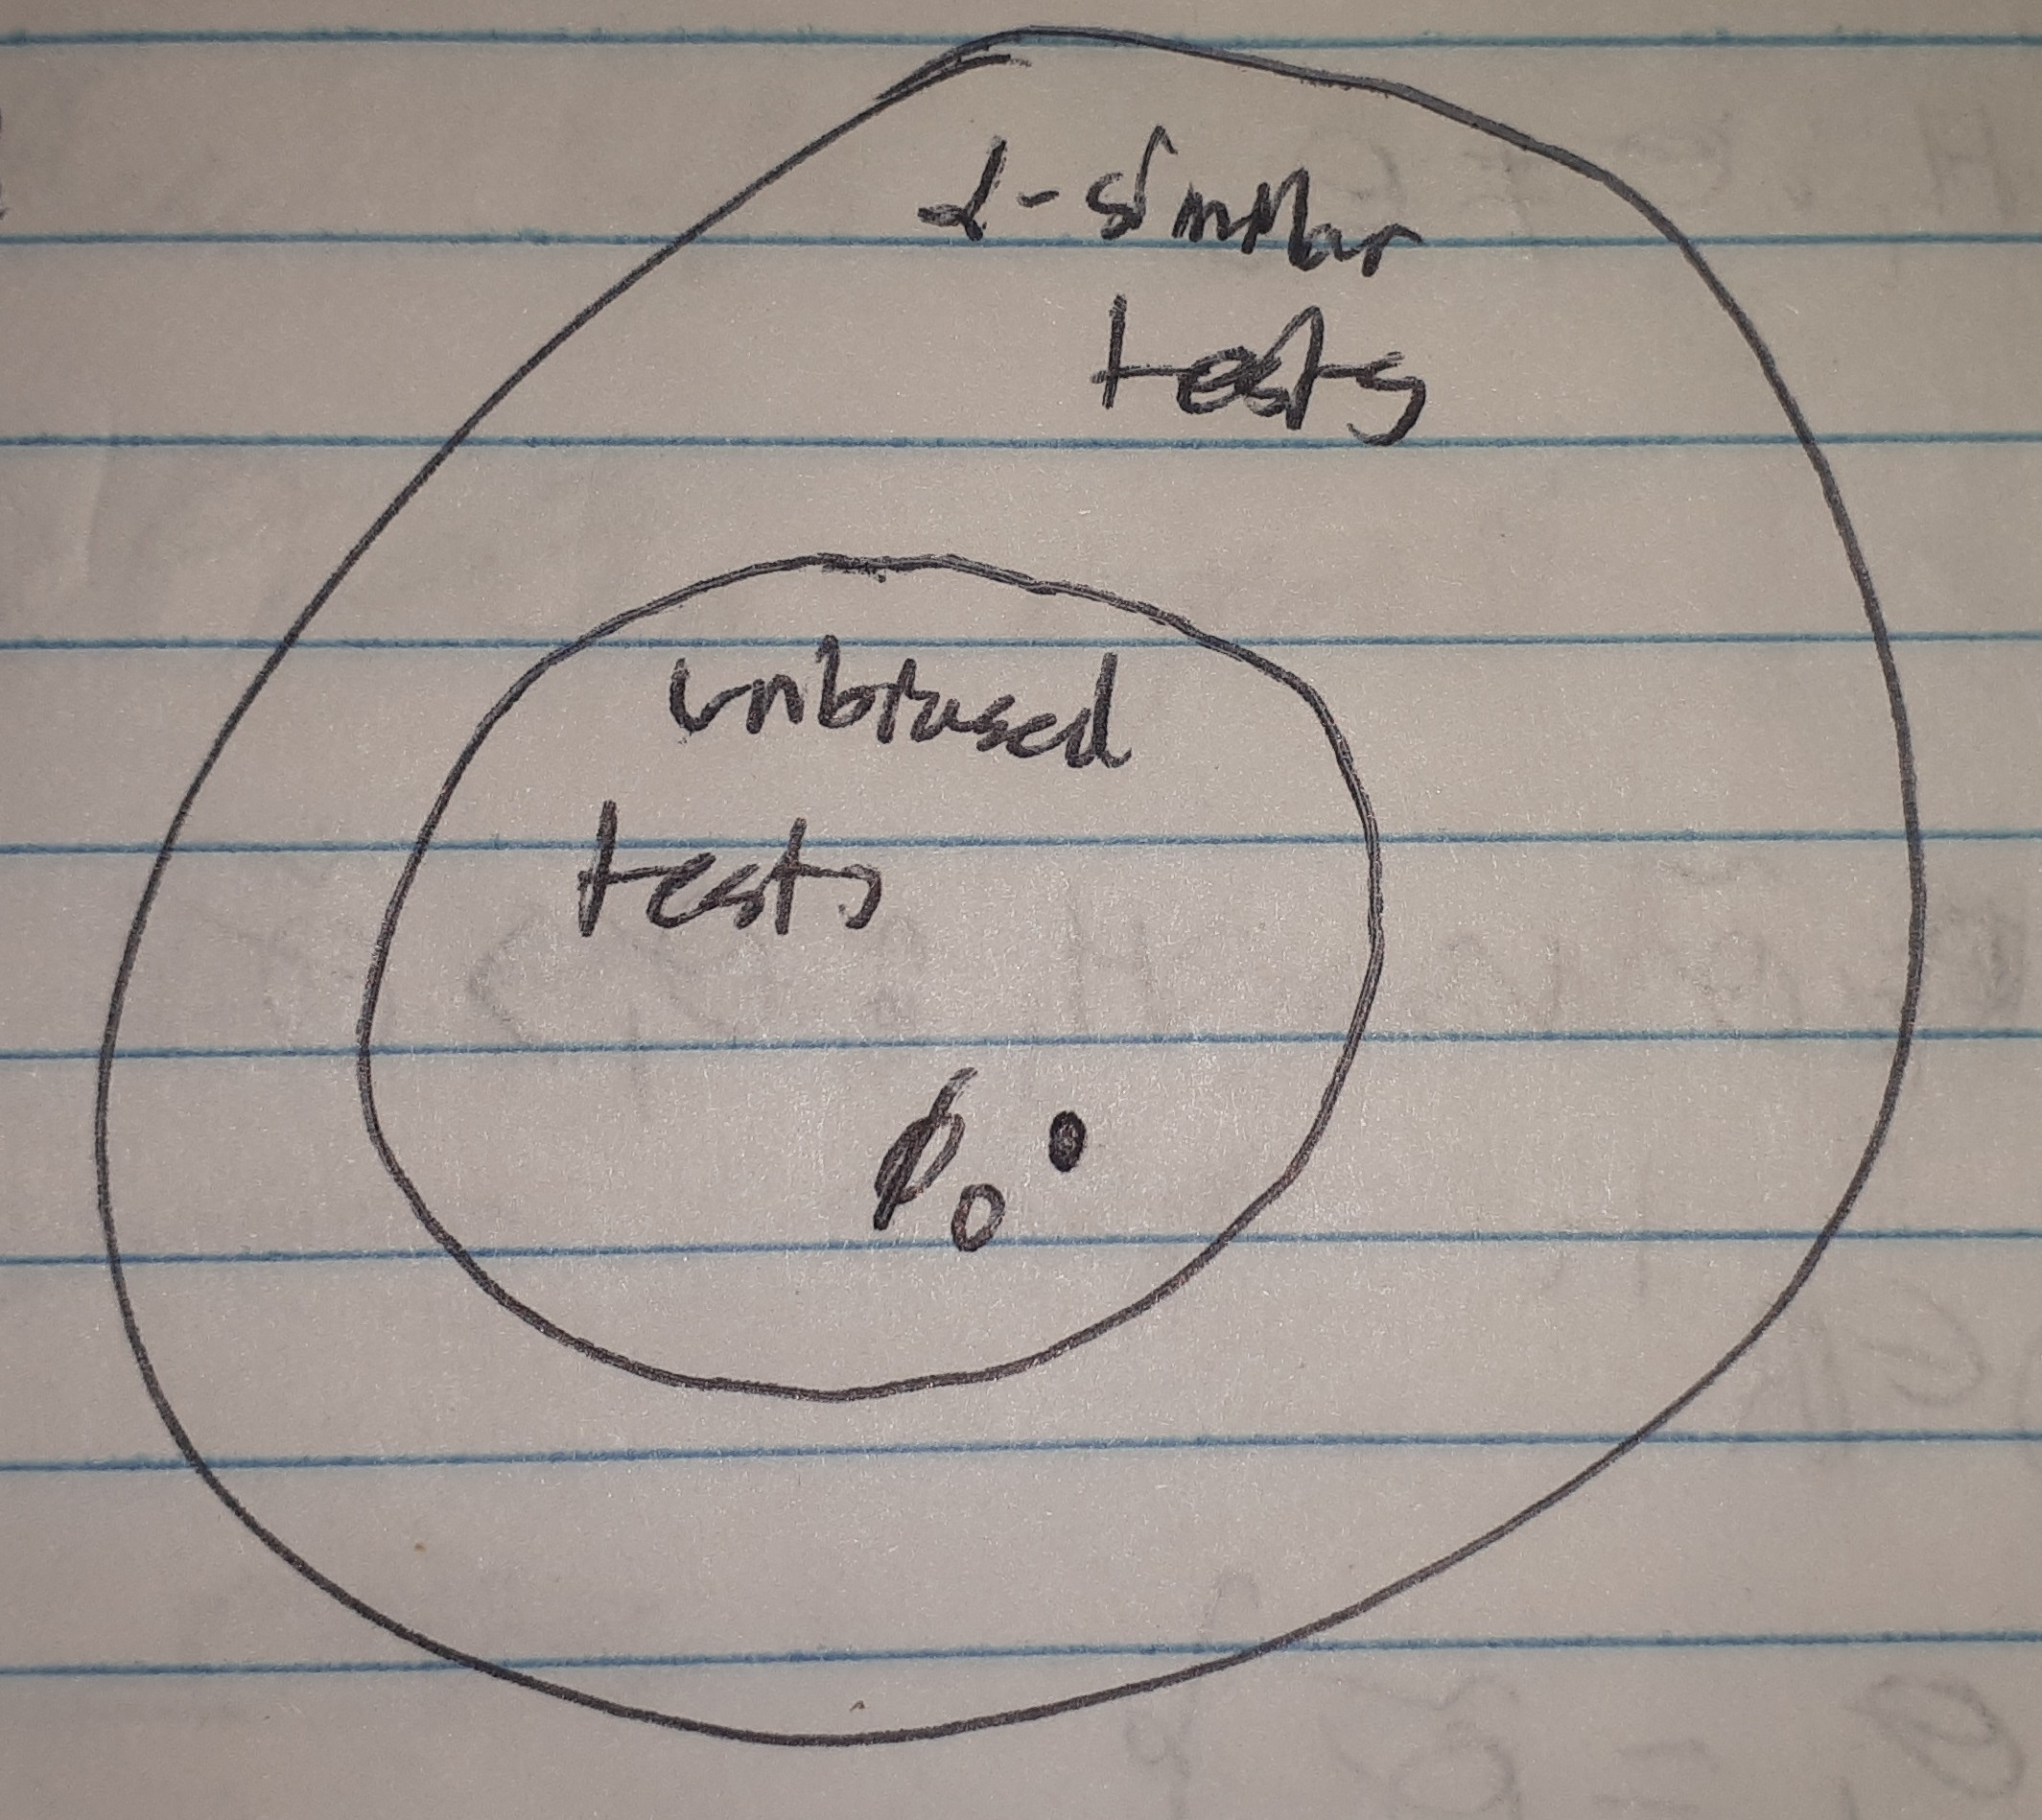
\includegraphics[width = 0.4\textwidth]{11_10_P2.jpg}
\end{center}
Thus a test which is UMP among $\al$-similar tests is UMP among unbiased tests.

\subsection{Method of undetermined multipliers}
We will now restrict our attention to one-dimensional exponential families so that 
\[p_\ta(x) = h(a)\exb{\ta T(x)-A(\ta)}.\]
We wish to test $H_0 : \ta=\ta_0$ against $H_1 :\ta \neq \ta_0$. Recall that no UMP test exists. One can show by the dominated convergence theorem that the map $\beta_\phi(\ta) = \E_\ta \phi$ is continuous and in fact differentiable for all test functions $\phi$. 

By our lemma from before we know that if $\phi$ is unbiased then $\E_{\ta_0}\phi = \al$ and $\E_\ta \phi \ge \al$ for all $\ta$. Thus every unbiased level $\al$ test must statisfy $\E_{\ta_0}\phi=\al$ and $\ta_0$ must be a global minimum of $\ta \mapsto \beta_\phi(\ta)$. So our power function looks something like this:

\begin{center}
    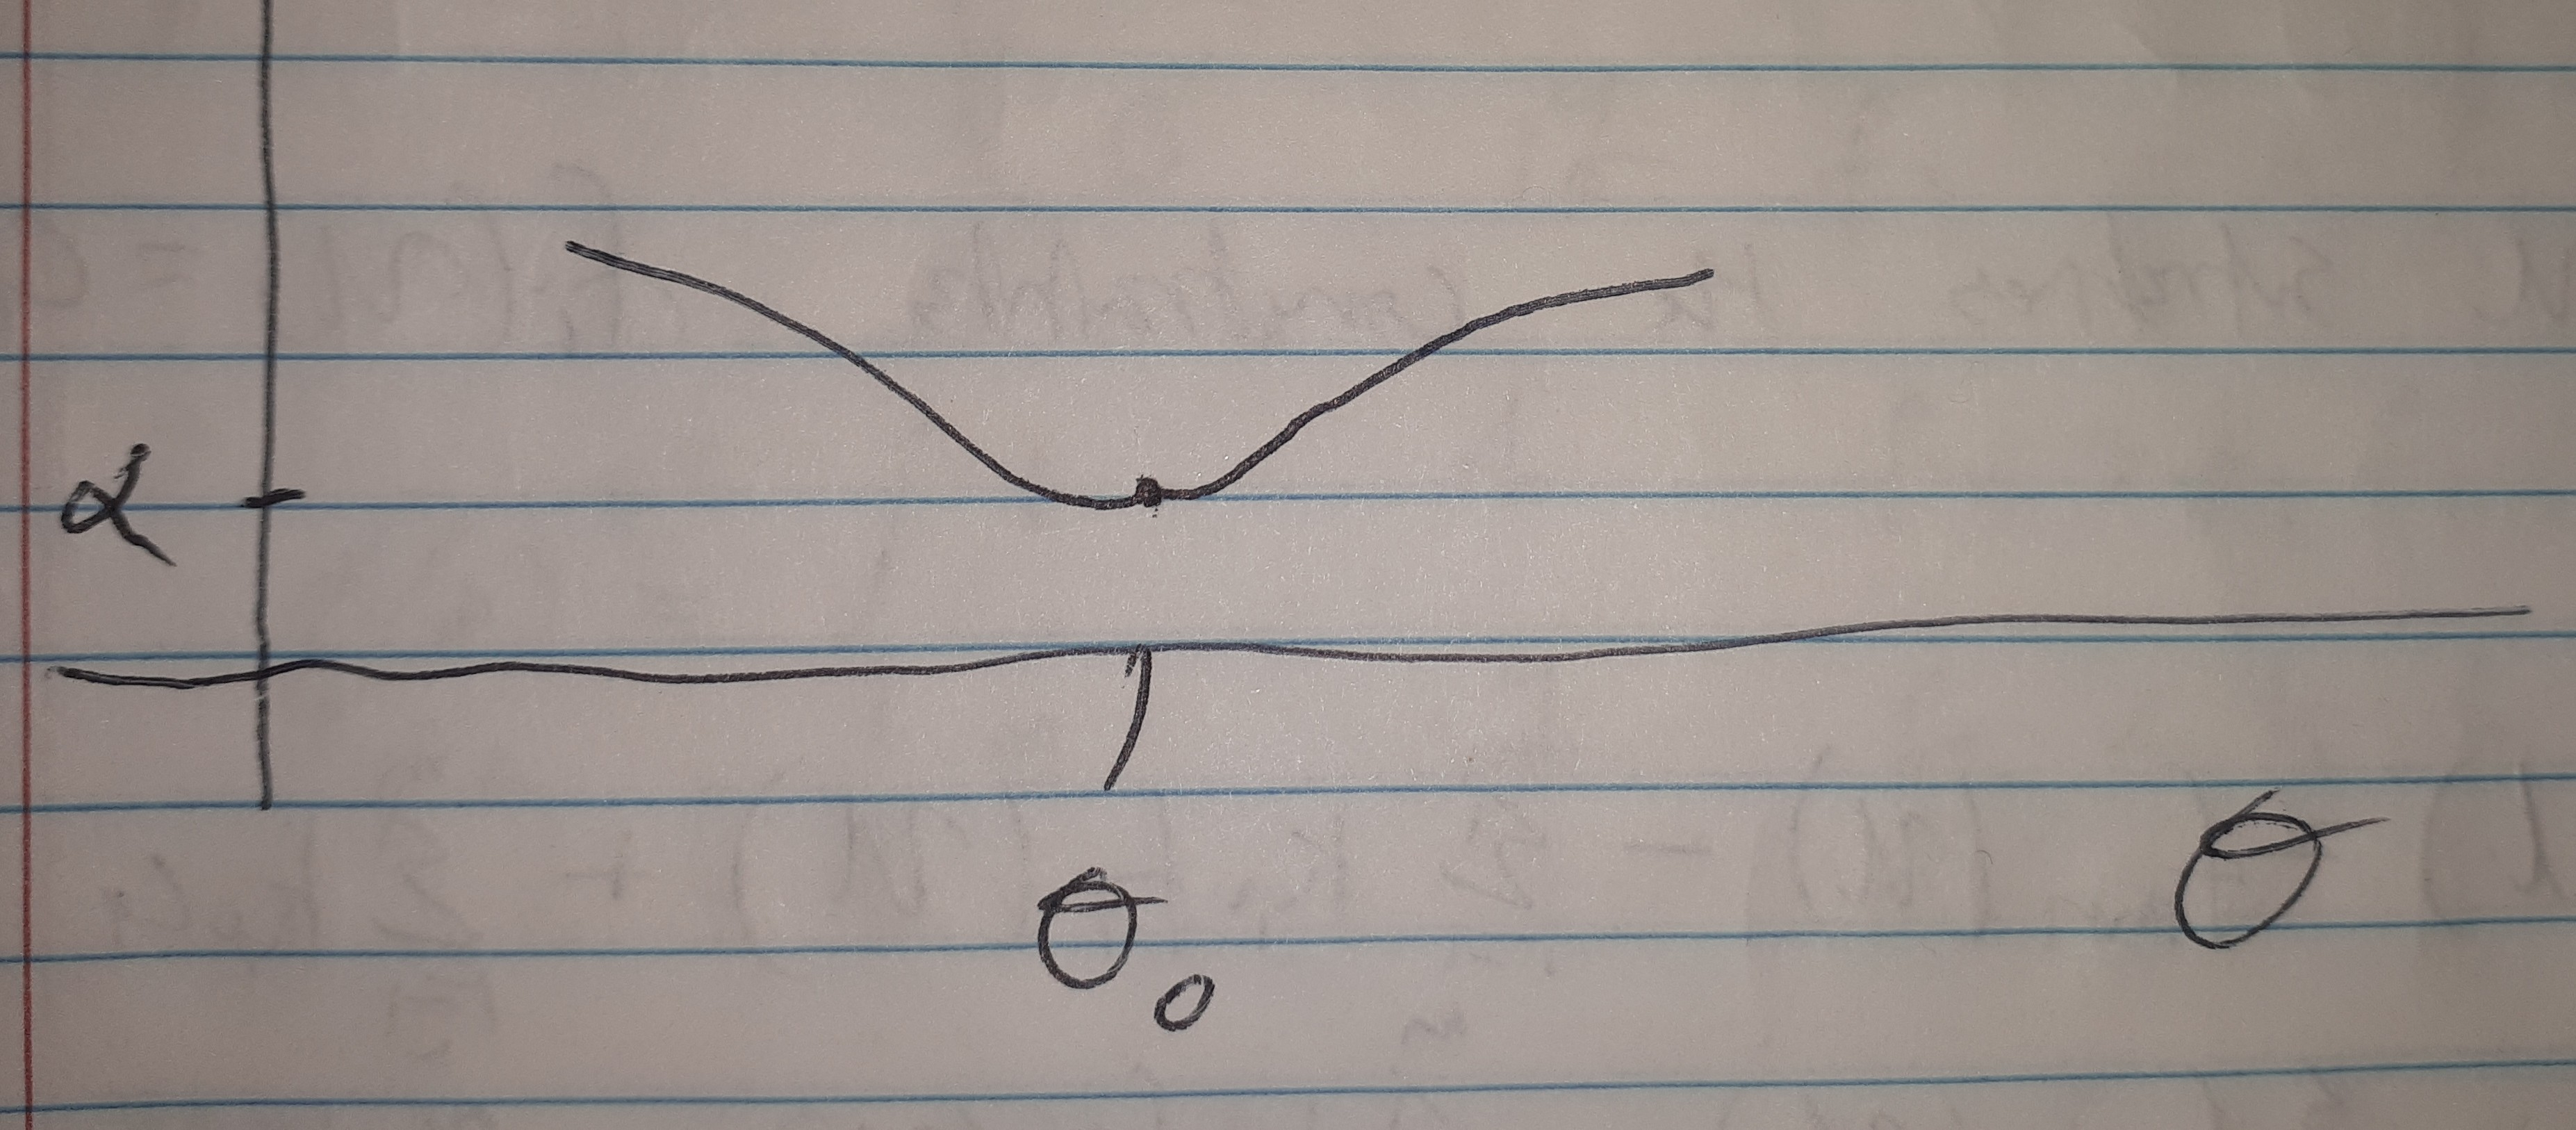
\includegraphics[width = 0.7\textwidth]{11_10_P3.jpg}
\end{center}


Thus the derivative of the power function at $\ta=\ta_0$ must be zero. Hence every unbiased test must satisfy the two constraints:
\begin{equation}\label{constrain}
    \int_\X \phi(x) p_\ta(x)d\mu(x) = \al ~~~\text{and}~~~ \partial_\ta \beta_\phi(\ta)\mid_{\ta = \ta_0} = \int_\X \phi(x) \partial_\ta p_{\ta_0}(x)d\mu(x) =0.
\end{equation}
In the second constrain we used some of the regularity properties of exponential families to exchange integration and differentiation. We will use the two above constraints to prove a generalized Neyman Pearson lemma which is called the method of undetermined multipliers. The method of undetermined multipliers is similar to the use of Lagrange multipliers in optimization. We will use the following general lemma.
\begin{lemma}[TSH Lemma 3.6.1]
    Suppose $f_1,\ldots,f_m,f_{m+1}$ are real valued functions on a space $U$ and that we want to maximize $f_{m+1}(u)$ subject to the constraints $f_i(u)=c_i$ for $i=1,\ldots,m$. If $u_0 \in U$ satisfies the the constaints $f_i(u_0)=c_i$ and there exist $k_1,\ldots,k_m \in \R$ such that $u_0$ maximizes
    \[f_{m+1}(u)-\sum_{i=1}^m k_if_i(u),\]
    over $U$, then $u_0$ maximizes the orginal optimization problem.
\end{lemma}
 
\begin{proof}
    Suppose we have such a $u_0$ and corresponding values of $k_i$. Let $u \in U$ satisfy the constaints $f_i(u)=c_i$. Then
    \begin{align*}
        f_{m+1}(u) &= f_{m+1}(u)-\sum_{i=1}^m k_i f_i(u) + \sum_{i=1}^m k_ic_i\\
        &\le f_{m+1}(u_0)-\sum_{i=1}^m k_i f_i(u_0) + \sum_{i=1}^m k_ic_i\\
        &= f_{m+1}(u_0).
    \end{align*}
    Thus $u_0$ maximizes $f_{m+1}(u)$ subject to $f_i(u)=c_i$.
\end{proof}
The coefficients $k_1,\ldots, k_m$ are called \emph{undetermined multipliers}. The idea is that for every choice of $k=(k_1,\ldots,k_m)$, solving the unconstrained optimization problem is easy and gives us a solution $u_0 = u_0(k)$. We then vary $k$ so that $u_0$ actually satisfies the constraints $f_i(u_0)=c_i$. This last step is often much harder than the unconstrained optimization. 
\subsection{UMPU tests for one-dimensional exponential families}
Returning to the setting of one-dimensional exponential families, our space $U$ is the set of all test functions $\phi : \X \to [0,1]$. For a fixed alternative we wish to maximize the power of $\phi$
\[f_3(\phi)=\E_{\ta_1}\phi = \int \phi(x)p_{\ta_1}(x)d\mu(x). \]
Subject to the constraints from equation \eqref{constrain}. Namely we want
\[f_2(\phi)=\int \phi(x)p_{\ta_0}(x)d\mu(x) = \al, \]
and
\[f_1(\phi) = \int \phi(x) \partial_\ta p_{\ta_0}(x)d\mu(x) = 0. \]
The constraint $f_2(\phi)=\al$ is sufficient for $\phi$ to be $\al$-similar and the constraint $f_1(\phi)=0$ is necessary for $\phi$ to be unbiased. For undetermined multipliers $k_1,k_2$, we wish to maximize
\begin{align}\label{multipliers}
    f_3(\phi)-k_1f_1(\phi)-k_2f_2(\phi) &= \int \phi(x)(p_{\ta_1}(x)-k_1p_{\ta_0}(x)-k_2\partial_\ta p_{\ta_0}(x))d\mu 
\end{align}
The test function $\phi$ is always in $[0,1]$. Thus any function $\phi_{k_1,k_2}$ satisfying
\begin{align}\label{k1k2}
    \phi_{k_1,k_2}(x) &=\begin{cases}
        1 &\text{if }p_{\ta_1}(x)-k_1p_{\ta_0}(x)-k_2\partial_\ta p_{\ta_0}(x)>0,\\
        0 & \text{if }p_{\ta_1}(x)-k_1p_{\ta_0}(x)-k_2\partial_\ta p_{\ta_0}(x)<0.
    \end{cases}\nonumber\\
    &=\begin{cases}
        1 &\text{if }p_{\ta_1}(x)>k_1p_{\ta_0}(x)+k_2\partial_\ta p_{\ta_0}(x),\\
        0 & \text{if }p_{\ta_1}(x)<k_1p_{\ta_0}(x)+k_2\partial_\ta p_{\ta_0}(x).
    \end{cases}
\end{align}
maximizes equation \eqref{multipliers}. Thus we wish to find $k_1,k_2$ and $\phi_{k_1,k_2}$ satisfying equation \eqref{k1k2} such that 
\begin{align*}
    \int \phi_{k_1,k_2} p_{\ta_0}d\mu &=\al \\
    \int \phi_{k_1,k_2} \partial_\ta p_{\ta_0} d\mu& =0.
\end{align*}
By the method of moments, such a test will be MP under the constraints \eqref{constrain}. Recall that 
\[p_\ta(x)=h(x)\exb{\ta T(x)-A(\ta)}, \]
and so 
\begin{align*} 
    \partial p_\ta(x)& = h(x)\exb{\ta T(x)-A(\ta)}(T(x)-A'(\ta))\\
    &=p_\ta(x)(T(x)-A'(\ta))\\
    &=p_\ta(x)(T(x)-\E_\ta[T(X)]),
\end{align*}
by previous results on exponential families. Thus the condition $p_{\ta_1}(x)>k_1p_{\ta_0}(x)+k_2\partial_\ta p_{\ta_0}(x)$ from \eqref{k1k2} is equivalent to
\[\frac{p_{\ta_1}(x)}{p_{\ta_0}(x)}=c\exb{(\ta_1-\ta_0)T(x)} > k_2+k_1(T(x)-\E_{\ta_0}[T(X)]), \]
where $c>0$ is a constant which does not depend on $x$. If we plot both $c\exb{(\ta_1-\ta_0)T(x)}$ and $k_2+k_1(T(x)-\E_{\ta_0}[T(X)])$ as functions of $T(x)$ we get a plot like the picture bellow. From this plot we can calculate the corresponding rejection region of $\phi_{k_1,k_2}$ (shown in red).

\begin{center}
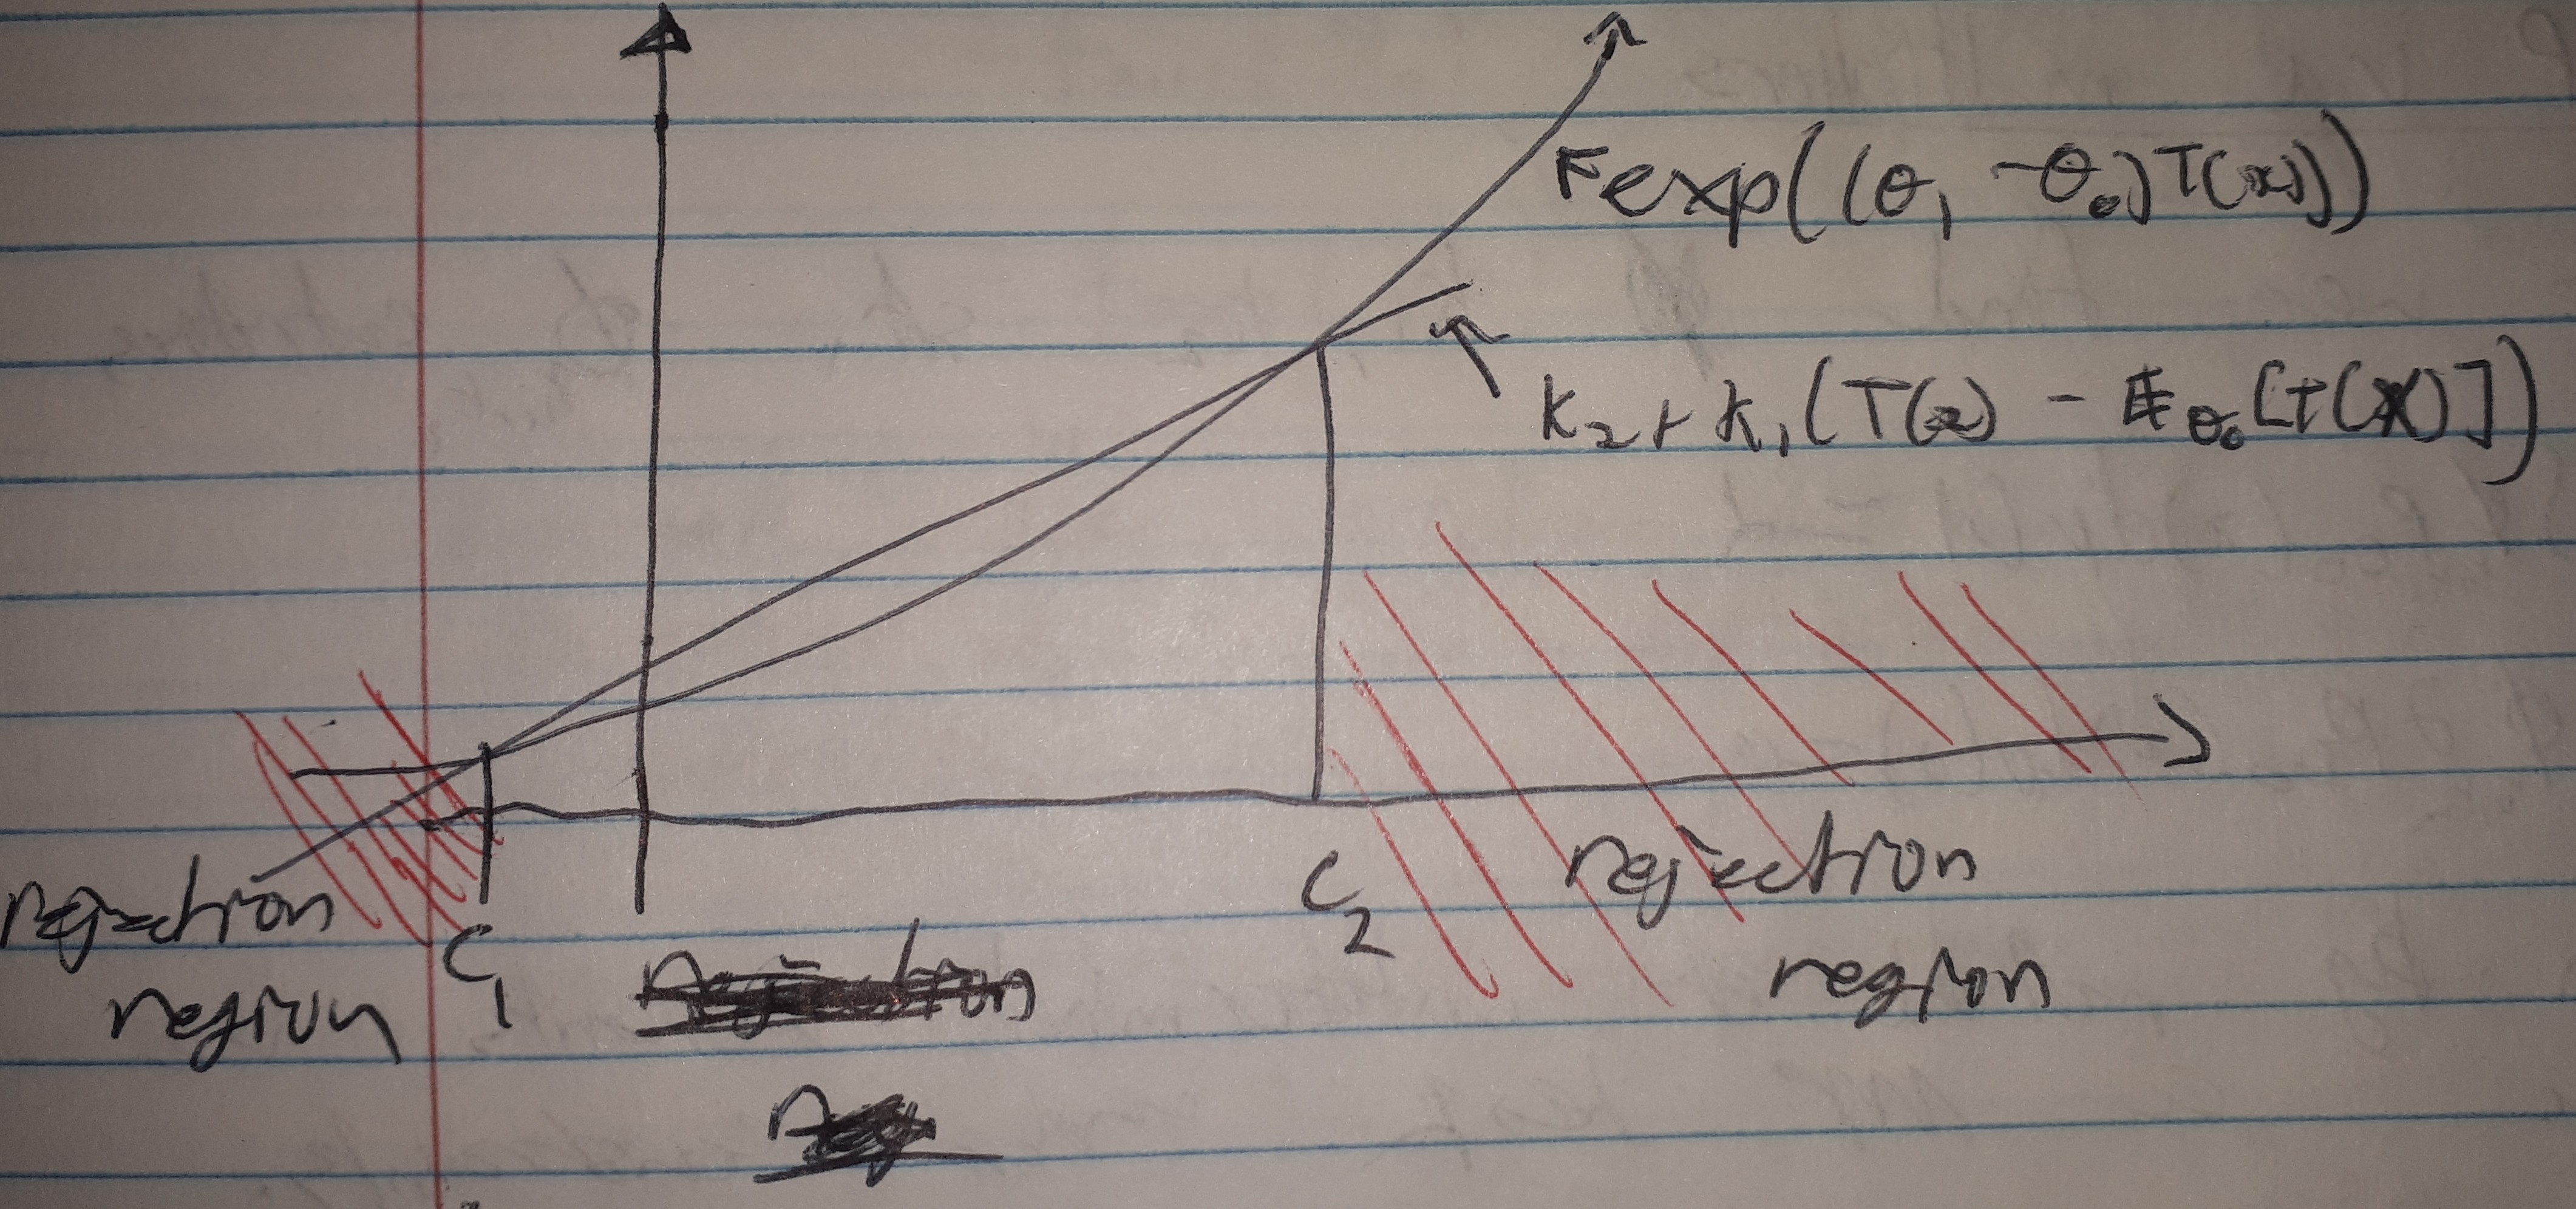
\includegraphics[width = 0.9\textwidth]{11_10_P4.jpg}
\end{center}

It is however possible that the two curves only intersect once in which case we would get a plot and rejection region that looks like this:

\begin{center}
    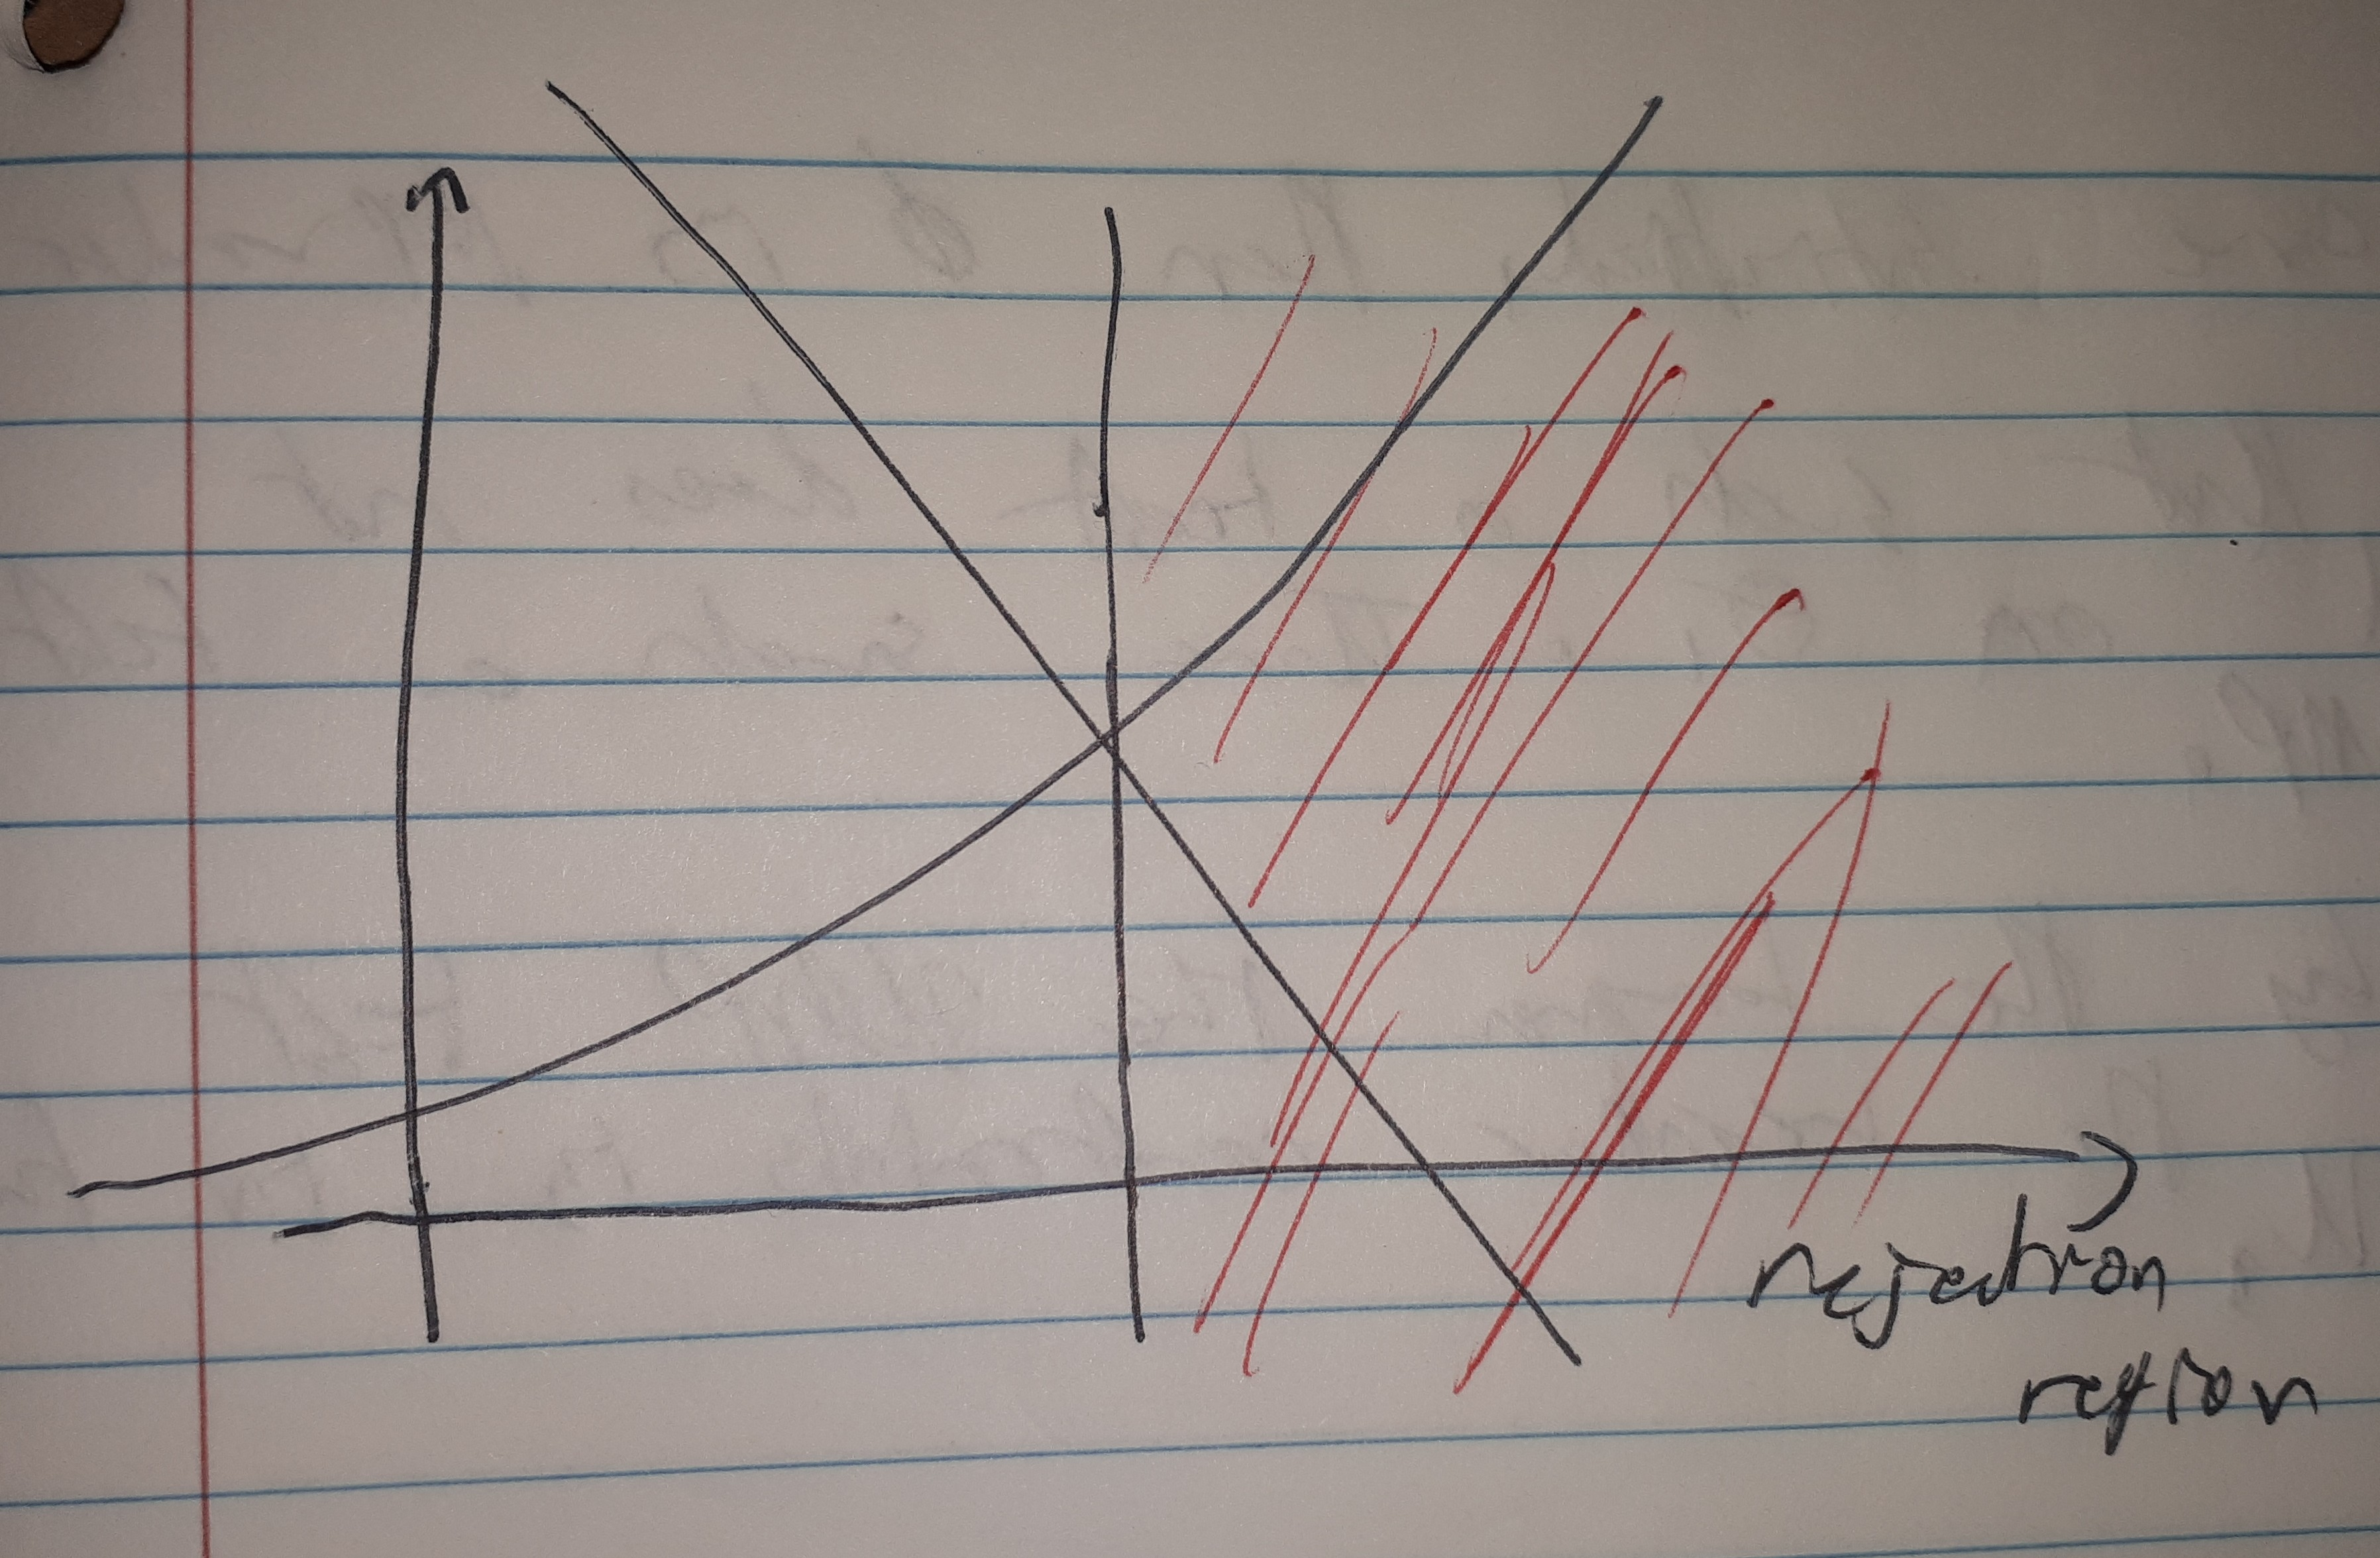
\includegraphics[width = 0.7\textwidth]{11_10_P5.jpg}
\end{center}
However, the above test is one-sided and thus will not satisfy the derivative constraint and hence will not be unbiased. Thus we know that we only need to consider tests where the curves intersect twice. We will thus reparametrize our problem 
\[(k_1,k_2) \longleftrightarrow (c_1,c_2), \]
where $c_1 \le c_2$ are the two values of $T(x)$ where the curves intersect. Under this parametrization our test will be
\begin{align*}
    \phi(x) & =\begin{cases}
        1 & \text{if } T(x) < c_1,\\
        \gamma_1 & \text{if } T(x) = c_1,\\
        0 & \text{if } c_1 < T(x) < c_2,\\
        \gamma_2 & \text{if } T(x) = c_2,\\
        1 & \text{if } T(x) > c_1.
    \end{cases}
\end{align*}
Using the method of moments we need to choose $c_1,c_2,\gamma_1,\gamma_2$ so that the constraints $f_2(\phi)=\al$ and $f_3(\phi)=0$ are met. Such a test will be MP under the constraints. Since the test $\phi$ does not depend on $\ta_1$ the test will be UMP under the constraints. Thus by our first lemma this test will also be UMPU. 
\end{document}